\documentclass[conference]{IEEEtran}
\IEEEoverridecommandlockouts
% The preceding line is only needed to identify funding in the first footnote. If that is unneeded, please comment it out.
\usepackage{cite}
\usepackage{amsmath,amssymb,amsfonts}
\usepackage{algorithmic}
\usepackage{graphicx}
\usepackage{textcomp}
\usepackage{xcolor}
\usepackage{graphicx}
\graphicspath{ {graphs/} }
\def\BibTeX{{\rm B\kern-.05em{\sc i\kern-.025em b}\kern-.08em
    T\kern-.1667em\lower.7ex\hbox{E}\kern-.125emX}}
\begin{document}

\title{Multi Agent PPO for Overcooked-AI Environment\\
}

\author{\IEEEauthorblockN{ Ryan Li}
\IEEEauthorblockA{ last commit: 1c80c54c52d9eceaf3366c40786a4860ef6bcac7}
}

\maketitle

\begin{abstract}
This paper will seek to explain Multi Agent PPO as a reinforcement learning approach to solving layouts of the Overcooked-AI environment. 
First, I will explain considerations behind the general direction of the project: which algorithms did I consider, and why I chose a different base algorithm
than what I went with in Project 2. Then, there will be an explanation of the Overcooked envinronment, and detailed analysis of the learning algorithm implemented. 
Lastly, I will outline the experiment details and discuss the results and how they relate to aspects of the algorithm. 
\end{abstract}

\section{General Direction}
In Project 2, I implemented a Deep Q Learning algorithm to solve the single agent Lunar Lander environment. The biggest difference for Project 3 is the 
multi agent aspect. I wanted to implement an algorithm that improves collaboration, and had explicit multi agent capabilities. I selected a different base algorithm for Project 3 called PPO 
with actor-critic policy network architecture. My main hypothesis is that two PPO agents with their own actor-critic networks can learn to collaborate
if we just give them shared rewards. 


\section{Environemnt Introduction}
The objective of Overcooked-AI is to cook and deliver as many onion soups as possible in 400 time step episodes. It is inspired by the 
popular video game, Overcooked. There are 2 agents, a discrete action space, and both agents have access to the full observation space. 
The MDP is fully-observable, making the state space equal to the observation space. There are different layouts to tackle, 
in this paper we will be looking at 5 of them. There are layouts that require coordination between the agents to be solved, implying that an 
explicit multi agent approach would be recommended. 

\section{Vanilla Policy Gradient: PPO Predecessor}

Before talking about PPO, it makes sense to talk about the basic Policy Gradient method in reinforcement learning, 
often known as Vanilla Policy Gradient. PPO is built upon Vanilla Policy Gradient, and can be viewed as an improved version. 
For Vanilla Policy Gradient, we define a policy network that represents the agent. It takes as input an observation vector, and 
outputs a probability distribution over the action space. Many people like to represent the policy network as a neural network. 
The goal then is to optimize the parameters of the neural network to achieve maximum expected reward. \par
The training protocol includes a rollout period where we step the environment, say for $n$ steps. We obtain $n$ observations, each observation is fed into
the Policy Network which outputs $n$ log probabilities of the possible actions. Each of the $n$ actions is sampled from its respective log probabilities.
In its simplest form, the loss function might look like:

\begin{equation}
    \mathbb{E}_{i}[A_i logp(y_i \vert x_i)]
\end{equation}

$A_i$ is the advantage can be calculated many ways, a common one is if we collect $r_t$ at every time step, we can use a discounted reward

\begin{equation}
    R_t = \sum_{k=0}^{\infty} \gamma^k r_{t+k}
\end{equation}

This advantage calculation says the magnitude to which we encourage or discourage actions is the weighted sum of all actions that come after. \par
Now, back to the loss function. We basically want to increase the log probabilities of actions that worked and decrease the log probabilities of actions
that did not work. For parameters $\theta$. For each sample there is the observation $x_i$, and an action $a_i$. We have a probaility distribution $p(x_i \vert \theta)$ from which 
we sampled $a_i$. The gradient that would lead to the increased probability of $a_i \vert x_i$ can be represented as $\nabla_\theta log p(x_i \vert \theta)$.
The advantage function is represented as $A_i$. Put together:

\begin{equation}
    \nabla_\theta log p(x_i \vert \theta) A_i
\end{equation}

The advantage function determines how strongly we nudge the parameters of the policy network in the direction of the gradient, hence Policy Gradient. 
If the advantage calculation of a certain action was positive and high, we nudge the parameters towards the positive gradient, increasing the log probability 
of that action being sampled again given similar observations. The opposite is true for large negative advantages, we nudge the parameters towards the 
negative gradient, decreasing log probability of the action. \par

\section{PPO Algorithm Analysis}
In the following sections I will discuss in detail the PPO algorithm implemented.

\subsection{Actor-Critic Approach}
In this implementation there is an Actor and Critic network per agent. Both networks are represented by neural networks constructed with PyTorch. 
Both take an observation as input, but the Actor Network returns a categorical probability distribution over the action space, while the Critic network
returns one value. Both networks have 2 hidden layers. 
The Actor Network controls which actions to take, and the Critic Network returns the value of the action taken. The Actor optimizes the
policy directly, while the Critic learns a value function. Actor-Critic combines the two common RL approaches, policy methods and value methods. 

\subsection{Generalized Advantage Estimation}
$\textit{Advantage}$ can be thought of as the advantage we gain by taking an action given a particular state. Recall that there are many ways
to calculate advantages, one we previously discussed was dicsounted returns. In this implementation we use Generalized Advantage Estimation. 
First we calculate a $\delta$

\begin{equation}
    \delta_i = reward_i + \gamma * value_{i+1} * nonterminal_{i+1} - value_i
\end{equation}

$\gamma$ is a discount factor. Reward is the reward at step $i$, and value is the output of the Critic network at step $i$. $nonterminal_i = 1 - done_i$. Nonterminal will 
equal zero if the game/episode is over, as we do not want to consider the next state if its from a new game. 
However, this is not an issue for Overcooked; it has a set horizon so each batch/ policy rollout contains one 400 step episode. 

\begin{equation}
    GAE_i = \delta_i + \gamma * \lambda * nonterminal_{i+1} * GAE_{i+1}
\end{equation}

$\lambda$ is a smoothing parameter used to reduce variance. The motivation for Generalized Advantage Estimation, is that in RL people
usually estimate long term reward/advantage with bootstrapped rewards from episodes, or a value function. Some data shows that GAE is better than both
because it reduces variance without introducing too much bias. 

\subsection{Clipped Policy Loss}
Perhaps the most important upgrade from Vanilla Policy Gradient to PPO, is the \textit{Clipped Objective}. The Vanilla Policy Gradient uses the 
log probability of the action to trace impact, but there are other way to do this. One way is to use probability of the action under the current 
policy divided by the probability of the action under the previous policy. It looks like:

\begin{equation}
    ratio_i = \frac{\pi_{new}(x_i \vert \theta)}  {\pi_{old}(x_i \vert \theta_{old})}
\end{equation}

Given this objective, if the current policy is more likely the $ratio_i$ will be greater than 1, and if the previous policy is more likely the 
$ratio_i$ will be between 0 and 1. The TRPO algorithm uses this function as loss. 
PPO further improves it by clipping:

\begin{equation}
    \mathbb{E}[max(-A_i * ratio_i, clip(ratio_i, 1- \epsilon, 1 + \epsilon) * -A_i)]
\end{equation}

If the current policy is much more likely, then $ratio_i$ will cause drastic updates in the gradient direction. 
Too large of updates can lead to divergent behaviors and cause instability. \textit{Clipped Objective} seeks to keep 
gradient steps at an appropriate magnitude to incerase stability. Here we choose to use the negative Advantage $-A_i$, depending 
on the implementation the positive $A_i$ is used to multiply the $ratio_i$. In that case it would be a $min$ function, but it achieves the same
purpose as what we have here.

\subsection{Total Loss}
The Total Loss is calculated as the Policy Loss - (Coefficient * Entropy Loss) + (Coefficient * Value Loss)

\begin{equation}
    PL - (Ecoeff * EL) + (Vcoeff * VL)
\end{equation}

For a categorical probability distribution $p$, the $\textit{entropy}$ is calculated as the mean of the natural log of the probabilities.

\begin{equation}
    \frac{1}{n} \sum_i^n ln(p_i)
\end{equation}

$\textit{Entropy}$ measures the uncertainty or randomness of a set of probabilities. Adding it as a bonus to the loss function 
encourages exploration and helps the algorithm not get stuck at local optima. \par
$\textit{Value}_i$ is the value returned by the Critic Network given observation $x_i$. The Value/Critic Loss is calculated as the mean squared error loss between the values
and returns in a given batch. The returns are the sum of the Values and the Advantages(Calculated by the Generalized Advantage Estimator)

\begin{equation}
    \frac{1}{n} \sum_i^n 0.5 * (Value_i - Return_i)^2
\end{equation}

After calculating the Total Loss, it is backpropagated and the optimizer is stepped to update parameters. 

\subsection{Training: Improved Policy Updating}
Because of the safeguards put in place by the $\textit{Clipped Objective}$, it is possible to run multiple training loops on samples
without causing instability. In this implementation, we run 400 steps of an Overcooked episode, collecting data each step. 
After episode termination/policy rollout, we do 4 epochs of training, each on randomly sampled data of size 100 from the policy rollout. This is also 
known as mini-batch updates. 

\subsection{Multi Agent Implementation}
To apply the actor-critic PPO implementation to this multi agent environment, I decided to go with what some call IPPO with shared rewards. 
Basically, each agent has its own actor-critic policy networks. At each time step each agent saves its owns observations, actions, values to its
own buffer. Importantly, the shaped rewards and reward returned by env.step are summed and given to each agent as a shared reward. After an episode
terminates, each agent calculates what is necessary from its own buffer and updates the parameters to its own actor-critif networks. This approach is
contrasted with what some call MAPPO, where the critic policy network is shared between the agents. I decided to implement IPPO with shared rewards 
because the relative simplicity of extending single agent PPO to multi agent IPPO meant if something went wrong the debugging process would be 
faster, and I could focus more on the training and analysis versus implementation. 

\section{Experiment}

\subsection{Setup and Procedure}
For each layout, we initialize two agents, each with their own buffer and actor-critic networks. For each step in an episode, each agent
inputs their respective observation into their actor network to get a categorical probability distribution of the action space. They receive log probabilities
from this distribution, and also sample this dsitribution for an action. Each agent also inputs their observation into their critic network to get 
a value estimation of the action. After stepping the env, done and rewards are shared. Reward shaping is turned on with the default values given 
by the instructor used, as well as adding the +20 for any soups made. We run 400 steps to collect 400 steps of data per episode. \par
After the data is collected the agents train separately. Per agent, sample 4 random mini batches, each size 100. For each minibatch calculate the advantages and returns using 
Generalized Advantage Estimator(GAE). We then can calculate Total Loss per agent, and update their respective Actor-Critic Networks. Each agent has 
one Adam optimizer that it shares between its Actor-Critic networks. \par
I train the agents on each layout for 25000 steps. 

\subsection{Tweaks and Different Attempts}
I tried reducing the shaped rewards to 1 for "placement in pot", "dish pickup reward", and 3 for "soup pickup reward" so that the 20 reward
for delivering a soup would have greater weight. This did not have a better effect than the default shaped rewards. I tried increasing the number of layers
in both the actor and critic networks for both agents. I expected this to increase total returns for the more complex maps as more layers can
capture more complexity, but actually returns decreased across the board. I implemented a linear decrease in shaped rewards, where the higher the
episode the less shaped rewards would be returned. This also had no discernable effect on my returns. Lastly I attempted to perform learning rate 
annealing. This had no discernable effect on my returns. 

\subsection{Training/Eval Results}
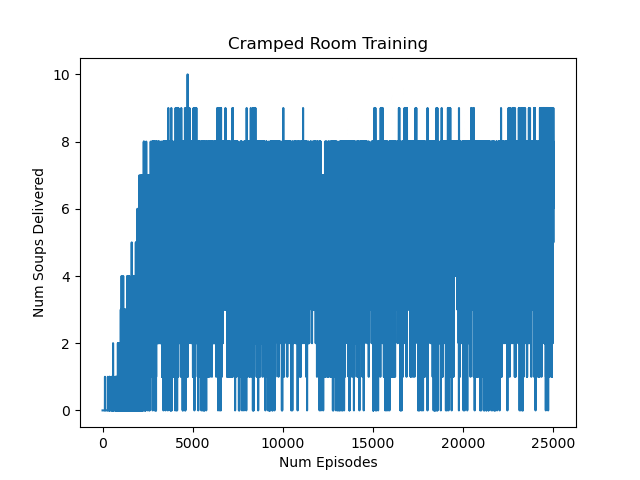
\includegraphics[scale=0.5]{crampedroom_training.png}
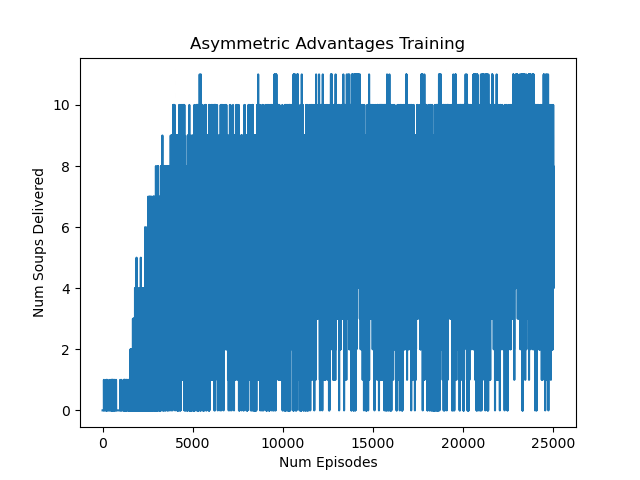
\includegraphics[scale=0.5]{assym_training.png}
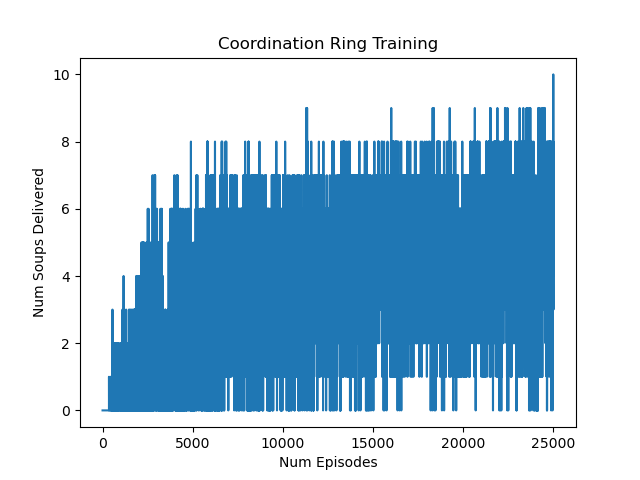
\includegraphics[scale=0.5]{coordring_training.png}
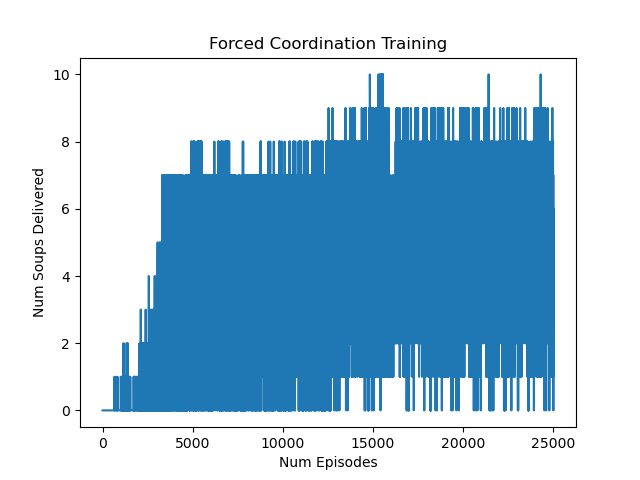
\includegraphics[scale=0.5]{forcedcoord_training.png}
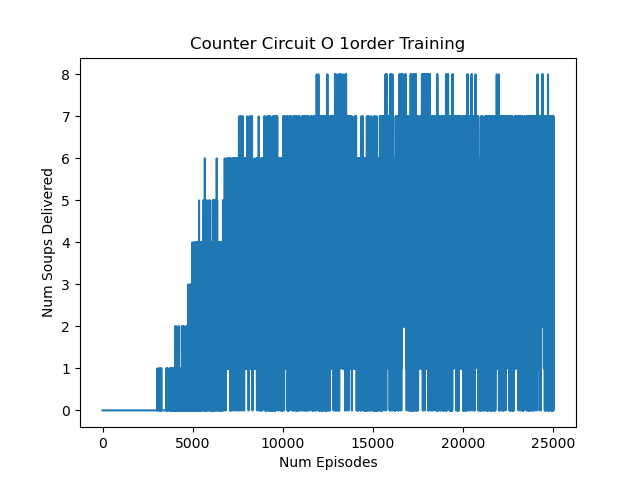
\includegraphics[scale=0.5]{countercircuit_training.png}
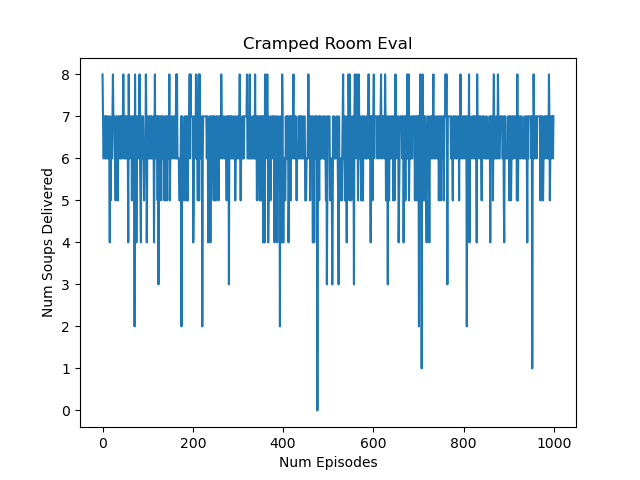
\includegraphics[scale=0.5]{crampedroom_eval.png}
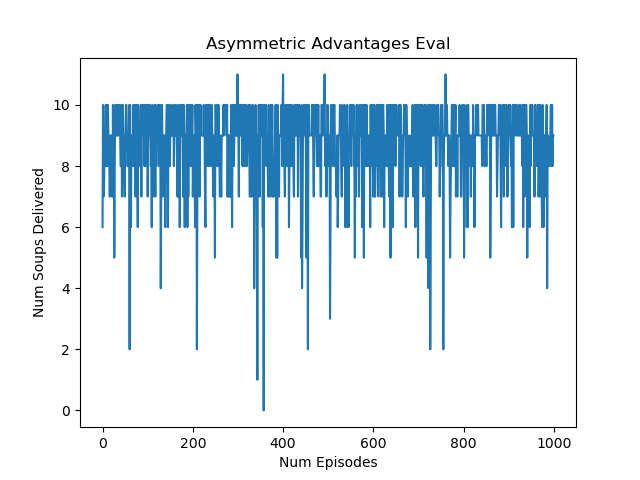
\includegraphics[scale=0.5]{asym_eval.png}
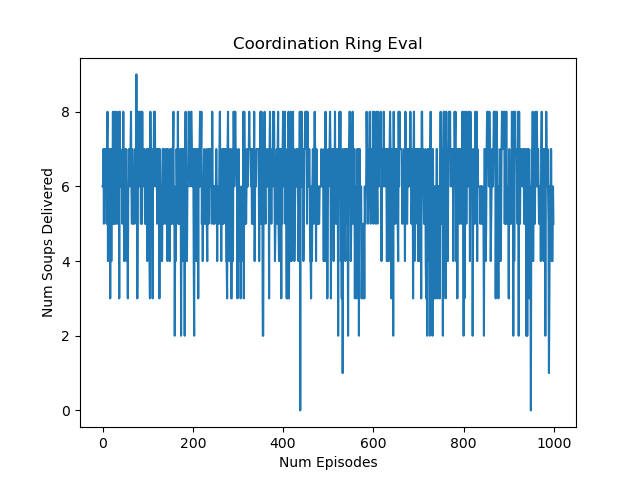
\includegraphics[scale=0.5]{coordring_eval.png}
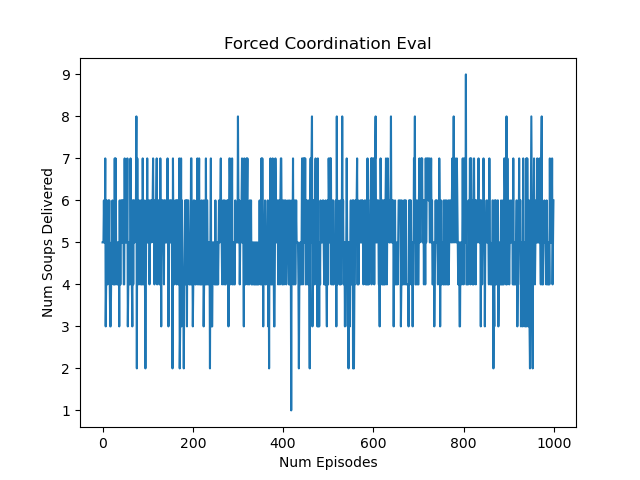
\includegraphics[scale=0.5]{forcedcoord_eval.png}
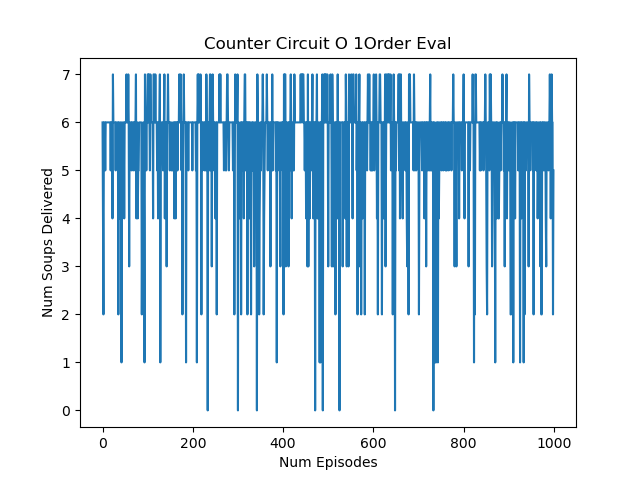
\includegraphics[scale=0.5]{countercircuit_eval.png}

For Training, the graphs show number of soups delivered for number of episodes trained for all 5 layouts. 
The graphs do show that the implemented Multi Agent IPPO algorithm was able to learn somewhat successfully for all 5 layouts. 
As the complexity of the layouts increases, the number of episodes needed to produce a single soup increases. At the same time, the number of episodes
needed to produce more soups after the initial soup also seems to take more time given the complexity. It is especially noticeable on 
layout 5, where it takes over 2000 episodes of training to produce a single soup. The layouts also seem to plateau, albeit at different times, where they do not 
gain more returns. On layouts 1 and 2, this could be a result of the 400 step horizon providing a hard limitation. But for layouts 3, 4, 5 the agents
should be able to achieve more than 7 soups consistently given the project description. I suspect this is because on the harder layouts there are 
vastly more possible trajectories and the agents settled into a local optima that wasn't the global optimum and could not "break out of it". I think 
one way to increase collaboration would be to implement a shared critic network. Some people call this decentrazlied execution and centralized training.
Unfortunately I was not able to successfully get this architecture to work, but I predict that it would have a better outcome than the IPPO approach.
A shared critic network would be able to take into account both agents actions, and influence its parameters in a way that encouraged collaboration.
Where as in my implementation, the main source of encouraging collaboraton is probably the shared rewards. \par
For Evaluation, the average soups over 1000 episodes were, cramped room: 6.339, asymmetric advantage: 8.703,  
coordination ring: 5.996, forced coordination: 5.073, counter circuit: 5.521. Only asymmetric advantage achieved more than 7 soups per episode.
The rest of the layouts were be able to achieve above 5, or close to 6 on average, which is not terrible. I believe these results are promising for 
this Multi Agent IPPO with shared rewards algorithm. With further hyperparamter tuning or additional techniques like better learning rate annealing, 
better mini batch selection in training, better reward horizon implementation, better fitting policy networks etc.,
this algorithm could achieve more than 7 soups in evaluation for all layouts I believe. 

\subsection{Other Metrics}
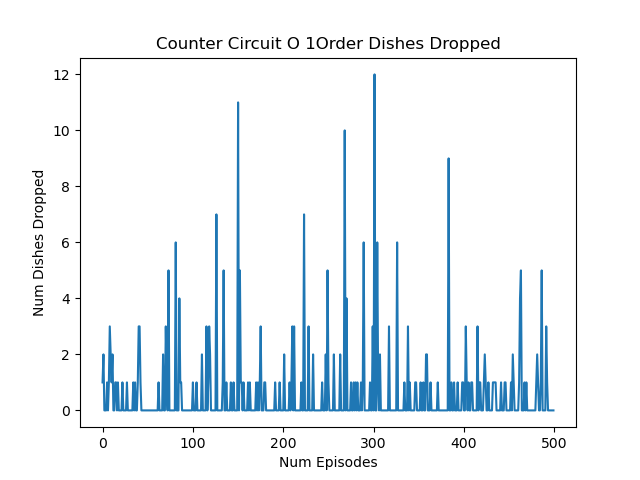
\includegraphics[scale=0.5]{counter_circuit_dishes.png}
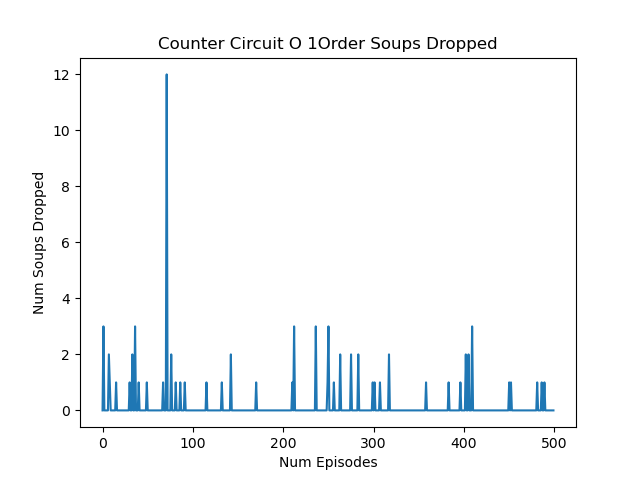
\includegraphics[scale=0.5]{counter_circuit_soups.png}
Other metrics that I was interested in involved sub tasks. Reward shaping was an important way to reward sub tasks that might lead up to the 
ultimate soup delivery. Without reward shaping the learning would converge much more slowly.
I was interested in if certain negative actions, like dropping dishes and soups should incur a negative reward. Many other environments 
have explicit negative rewards, and intuitively dropping a soup should probably be a negative reward for the agent. In terms of my algorithm, since
I have shared rewards, it seems that sharing negative rewards could discourage one agent from positive actions even though they did not do anything 
wrong. I regrettably did not have enough time to test this out, as I was mainly focused on improving algorithm techniques and tuning hyperparameters.
But I think experimenting with different negative rewards with IPPO and MAPPO would be very interesting. 

\section{Pitfalls and Problems}
A problem I encountered was difficulty experimenting given long training time. This environment was not compatible with OpenAI Gym's vectorization
module. Although it might have been feasible to provide one's own wrapper, I found it hard to test different hyper parameters, techniques and reward shapings
given lack of vectorization and my limited hardware. 

\end{document}
